
\begin{figure}
\begin{subfigure}{.5\linewidth}
\centering

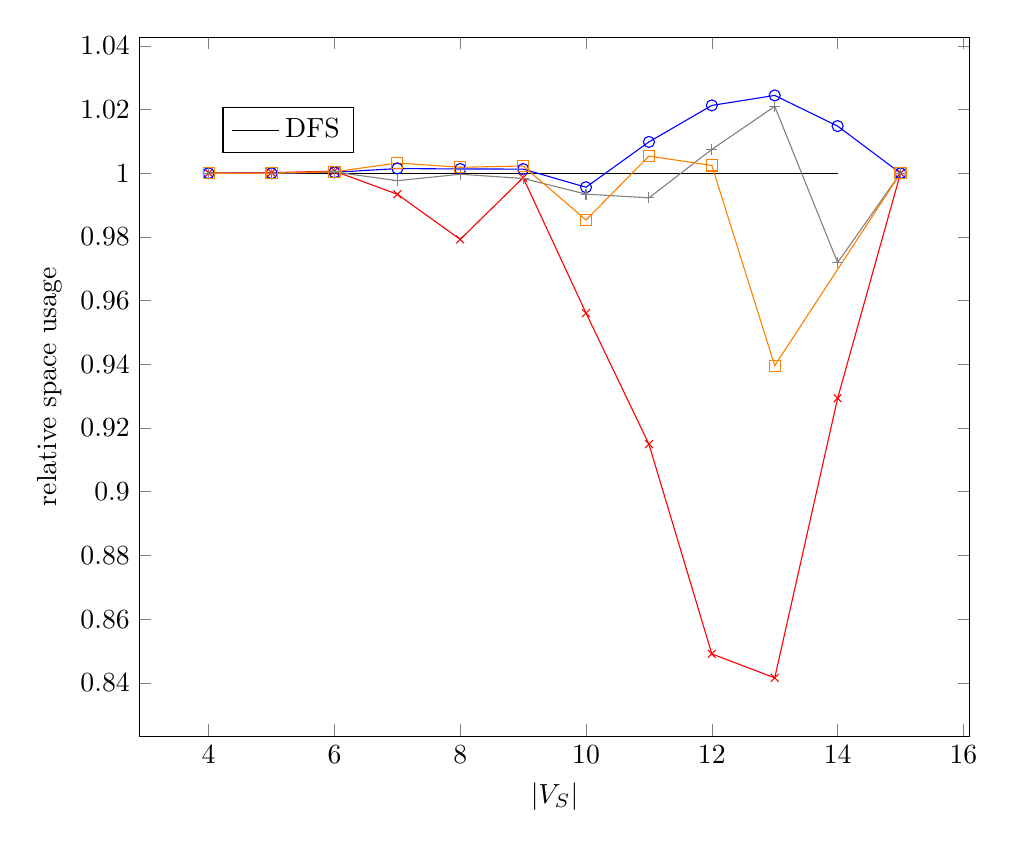
\begin{tikzpicture}
    \begin{axis}[
        xlabel=$|V_S|$,
        ylabel=relative space usage,
        legend style={at={(0.1,0.9)},anchor=north west},
        width=\textwidth,
		%y tick label style={/pgf/number format/sci},
    ]
\addplot [mark=none, black] plot coordinates {
        (4,1) (14,1)};
%\addlegendentry{Reference line}
   


\addplot[
        mark=x,
        red,
    ] plot coordinates {
        (4,1.0000965810314855)
        (5,1.000175389022596)
        (6,1.0006580115517583)
        (7,0.9933995199650884)
        (8,0.9792110986760141)
        (9,0.9985983790932417)
        (10,0.956082748149554)
        (11,0.9149464001158917)
        (12,0.8490897589091164)
        (13,0.8415538203024612)
        (14,0.929342492639843)
        (15,1.0)
};
%    \addlegendentry{DFS}


\addplot[
        mark=o,
        blue,
    ] plot coordinates {
        (4,1.0)
        (5,1.0)
        (6,1.0002820435514146)
        (7,1.0014677156516765)
        (8,1.0013303474424071)
        (9,1.0012937629376293)
        (10,0.9955989241814666)
        (11,1.0098277290517956)
        (12,1.0212860310421286)
        (13,1.0244208763605918)
        (14,1.014792899408284)
        (15,1.0)
};
%    \addlegendentry{DFS}

\addplot[
        mark=+,
        gray,
    ] plot coordinates {
        (4,1.0)
        (5,1.0)
        (6,1.000384959527228)
        (7,0.9976584694602273)
        (8,0.9996798586962521)
        (9,0.9983508509609041)
        (10,0.9934327298544551)
        (11,0.992267743796884)
        (12,1.0074733487196394)
        (13,1.0209750566893423)
        (14,0.971953578336557)
        (15,1.0)
};
  %  \addlegendentry{DFS}
  
  \addplot[
        mark=square,
        orange,
    ] plot coordinates {
        (4,1.0)
        (5,1.0)
        (6,1.0004306632213609)
        (7,1.0032082760426897)
        (8,1.0018603365614602)
        (9,1.0022712559935922)
        (10,0.9853084218205398)
        (11,1.0053814661276617)
        (12,1.0024461839530332)
        (13,0.9395811877789221)
%        (14,1.7399193548387097)
        (15,1.0)
};
    \addlegendentry{DFS}

   

    \end{axis}
    \end{tikzpicture}


\caption{Serial}
\end{subfigure}%
\begin{subfigure}{.5\linewidth}
\centering

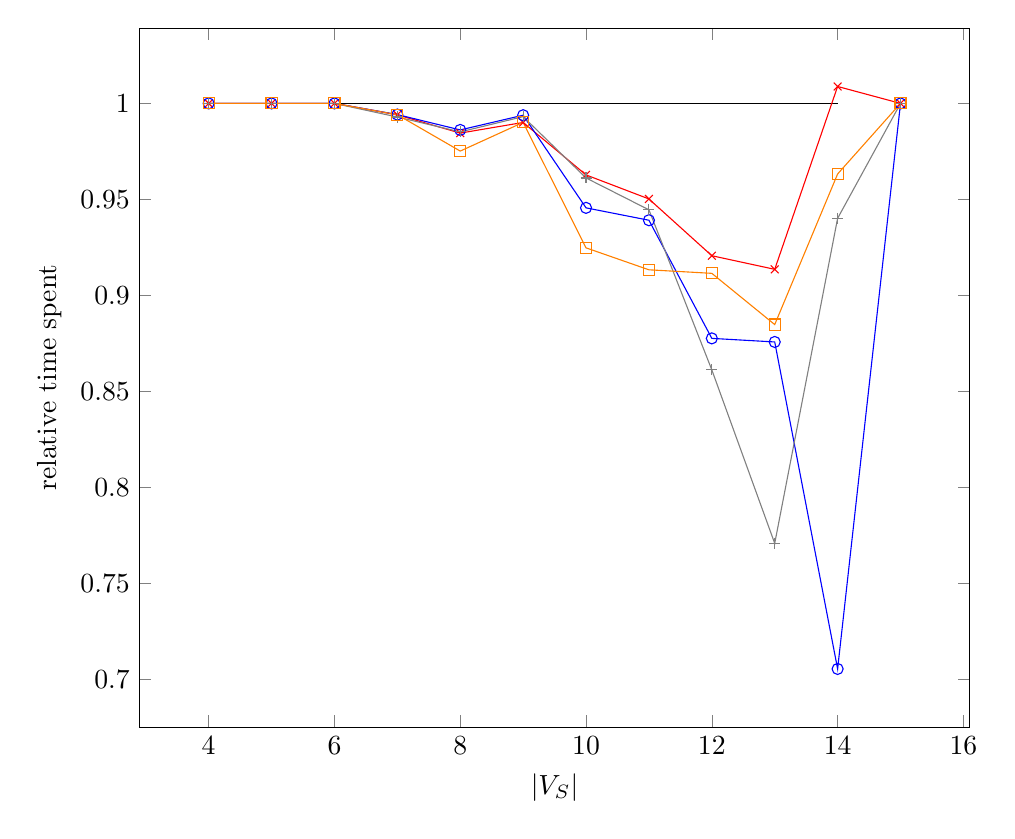
\begin{tikzpicture}
    \begin{axis}[
        xlabel=$|V_S|$,
        ylabel=relative time spent,
        %ymode=log,
        %legend style={at={(0.1,0.9)},anchor=north west},
        width=\textwidth,
		%y tick label style={/pgf/number format/sci},
    ]
\addplot [mark=none, black] plot coordinates {
        (4,1) (14, 1)};


  \addplot[
        mark=x,
        red,
    ] plot coordinates {
        (4,1.0)
        (5,1.0)
        (6,1.0)
        (7,0.9940409204420008)
        (8,0.9845363571451409)
        (9,0.9900799966049186)
        (10,0.9627679146352681)
        (11,0.9502480408368682)
        (12,0.9206893922062076)
        (13,0.9136043360433604)
        (14,1.0088148873653282)
        (15,1.0)
};
%    \addlegendentry{DFS}


\addplot[
        mark=o,
        blue,
    ] plot coordinates {
        (4,1.0)
        (5,1.0)
        (6,1.0)
        (7,0.9941864854662137)
        (8,0.9861872032406946)
        (9,0.9938485873720286)
        (10,0.9456110708826132)
        (11,0.9391634980988594)
        (12,0.8776561026905504)
        (13,0.8757868233319346)
        (14,0.7055435565154787)
        (15,1.0)
};
%    \addlegendentry{DFS}


\addplot[
        mark=+,
        gray,
    ] plot coordinates {
        (4,1.0)
        (5,1.0)
        (6,1.0)
        (7,0.9929013128162167)
        (8,0.9851651539867965)
        (9,0.9931084715374272)
        (10,0.9611769201375621)
        (11,0.9445889650906841)
        (12,0.8612382897795309)
        (13,0.7709207823524158)
        (14,0.9401544401544402)
        (15,1.0)
};
%    \addlegendentry{DFS}

\addplot[
        mark=square,
        orange,
    ] plot coordinates {
        (4,1.0)
        (5,1.0)
        (6,1.0)
        (7,0.9940991852791332)
        (8,0.9751758636861029)
        (9,0.9901049034841563)
        (10,0.92478721195765)
        (11,0.9133579589382356)
        (12,0.9115188281423393)
        (13,0.8848523475674527)
        (14,0.9632495164410058)
        (15,1.0)
};
%    \addlegendentry{DFS}
  

	
    \end{axis}
    \end{tikzpicture}

\caption{Cached}

\end{subfigure}\\[1ex]
\begin{subfigure}{0.5\linewidth}
\centering

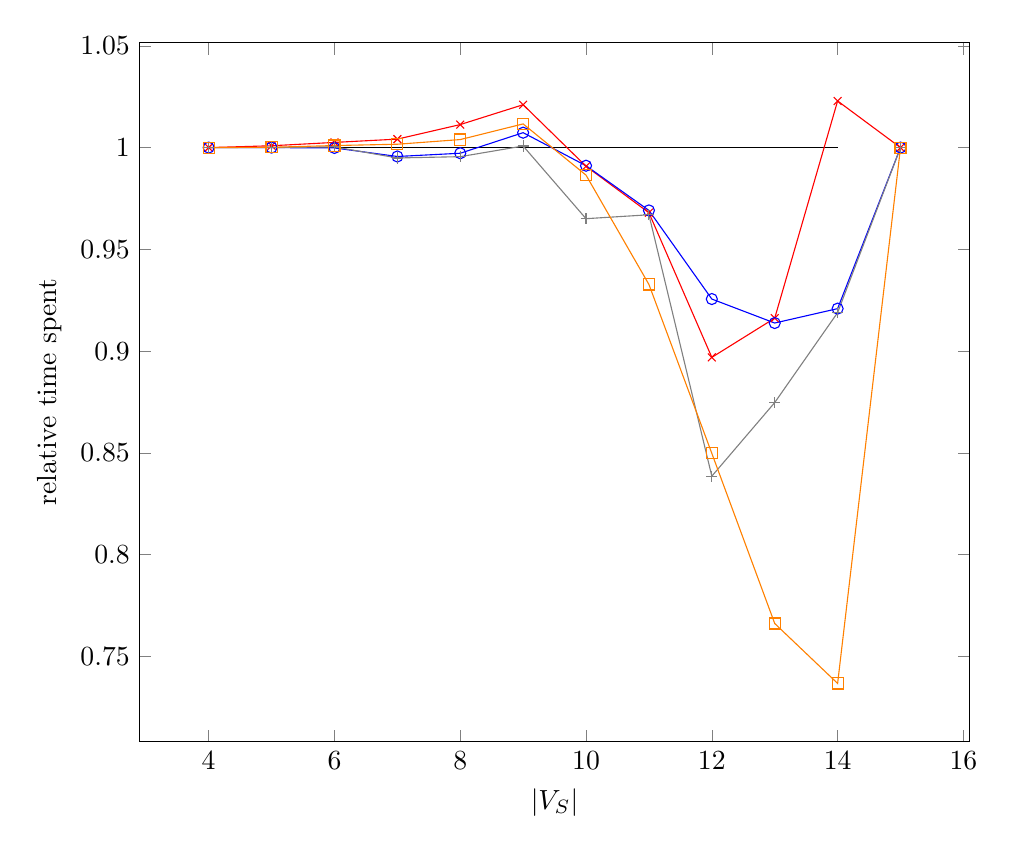
\begin{tikzpicture}
    \begin{axis}[
        xlabel=$|V_S|$,
        ylabel=relative time spent,
        %ymode=log,
        %legend style={at={(0.9,0.1)},anchor=south east},
        width=\textwidth,
		%y tick label style={/pgf/number format/sci},
    ]
\addplot [mark=none, black] plot coordinates {
        (4,1) (14, 1)};



\addplot[
        mark=x,
        red,
    ] plot coordinates {
        (4,1.0)
        (5,1.000900574605754)
        (6,1.0025478929245333)
        (7,1.0041639014364925)
        (8,1.0113109470838963)
        (9,1.0210621830797972)
        (10,0.9908368657511993)
        (11,0.9679989223930572)
        (12,0.896964856230032)
        (13,0.9162158413094743)
        (14,1.0229083665338645)
        (15,1.0)
};
%    \addlegendentry{DFS}


\addplot[
        mark=o,
        blue,
    ] plot coordinates {
        (4,1.0)
        (5,1.0)
        (6,0.9998377413597274)
        (7,0.9956367369636823)
        (8,0.9972272775934055)
        (9,1.0073297762880147)
        (10,0.9910981075697212)
        (11,0.9691430269928849)
        (12,0.9256116207951071)
        (13,0.9138302455838001)
        (14,0.9209039548022598)
        (15,1.0)
};
%    \addlegendentry{DFS}


\addplot[
        mark=+,
        gray,
    ] plot coordinates {
        (4,1.0)
        (5,1.0)
        (6,1.000354588972283)
        (7,0.9949073174942276)
        (8,0.995546811368853)
        (9,1.0007862470515736)
        (10,0.9650804809463783)
        (11,0.9670087167604546)
        (12,0.8386056820471489)
        (13,0.874765966299147)
        (14,0.9189443920829407)
        (15,1.0)
};
%    \addlegendentry{DFS}

\addplot[
        mark=square,
        orange,
    ] plot coordinates {
        (4,1.0)
        (5,1.000160404218631)
        (6,1.0010048031800365)
        (7,1.0016524520255863)
        (8,1.0039461691062141)
        (9,1.0116352465914829)
        (10,0.9864754590183608)
        (11,0.9327775946247194)
        (12,0.8498140635564571)
        (13,0.7662451575177253)
        (14,0.7368035190615836)
        (15,1.0)
};
%    \addlegendentry{DFS}




	
	
    \end{axis}
    \end{tikzpicture}

\caption{Parallel}
\end{subfigure}
\begin{subfigure}{.5\linewidth}
\centering

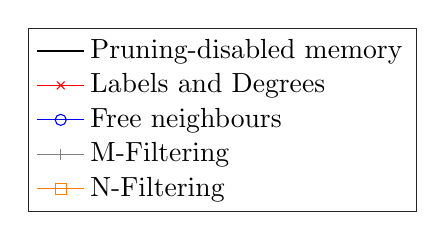
\begin{tikzpicture} 
    \begin{axis}[%
    hide axis,
    xmin=10,
    xmax=50,
    ymin=0,
    ymax=0.4,
    legend style={draw=white!15!black,legend cell align=left}
    ]
	\addlegendimage{black}
    \addlegendentry{Pruning-disabled memory}; 
     
    \addlegendimage{red, mark=x}
    \addlegendentry{Labels and Degrees};
    
    \addlegendimage{blue, mark=o}
    \addlegendentry{Free neighbours};
    
    \addlegendimage{gray, mark=+}
    \addlegendentry{M-Filtering};
    
    \addlegendimage{orange, mark=square}
    \addlegendentry{N-Filtering};
    
    
    \end{axis}
\end{tikzpicture}


\caption{Serial}

\end{subfigure}%

\caption{Memory usage of our algorithm with \textbf{AllDifferent} pruning using various filtering methods compared to memory usage without pruning. We avoid unnecessarily long paths, do not perform contraction, use the degree-based target vertex ordering and use DFS path iteration. Data points above the black reference line denote that the pruning method increases memory usage and data points below the reference line denote that the pruning method saves memory.}	
\label{fig:spaceAllDifferent}
\end{figure}
